%%%%%%%%%%%%%%%%%%%
% File: Manual_Module_2_Cyclic_improved.tex
% English manual for module 2 of the cyclic part of the mol-infer project
% Edit: Feb 9, 2021
%%%%%%%%%%%%%%%%%%%

\documentclass[11pt, titlepage, dvipdfmx, twoside]{article}
\linespread{1.1}
%\documentclass[11pt,dvipdfmx,twoside]{jarticle}
%%%%%%%%%%%%%%%%%%%%%%%%%%%%%%%%%%%%%%%%%%%%%%%%%%%%%%%%%%%%%%%%%%%%%%%%%%%%%%
% style definitions
%
% following setting makes 3cm spaces for top and bottom, and
% 2.5cm spaces for left and right
%
                                         % default setting
\setlength{\oddsidemargin}{22pt}         % 62pt
\setlength{\evensidemargin}{22pt}        % 62pt
\setlength{\headheight}{12pt}            % 12pt
\setlength{\textheight}{662pt}           % 592pt
\setlength{\marginparsep}{10pt}          % 10pt
\setlength{\footskip}{30pt}              % 30pt
\setlength{\hoffset}{-13pt}              % 0pt
\setlength{\paperwidth}{597pt}           % 597pt
\setlength{\topmargin}{20pt}             % 20pt
\setlength{\headsep}{25pt}               % 25pt
\setlength{\textwidth}{427pt}            % 327pt
\setlength{\marginparwidth}{106pt}       % 106pt
\setlength{\marginparpush}{5pt}          % 5pt
\setlength{\voffset}{-37pt}              % 0pt
\setlength{\paperheight}{845pt}          % 845pt


% 1 inch = 2.54 cm = 72.27 pt

\renewcommand{\baselinestretch}{1.20}

%%%%%%%%%%%%%%%%%%%%%%%%%%%%%%%%%%%%%%%%%%%%%%%%%%%%%%%%%%%%%%%%%%%%%%%%%%%%%%
\usepackage{amsfonts}
\usepackage{amssymb}
\usepackage{amsmath}
\usepackage[dvipdfmx]{graphicx}
\usepackage{framed}
\usepackage{url}
\usepackage{color}

%%%%%%%%%%%%%%%%%%%%%%%%%%%%%%%%%%%%%%%%%%%%%%%%%%%%%%%%%%%%
\newcommand{\project}{{\tt mol-infer/Cyclic\_improved}}
%\newcommand{\project}{{\tt mol-infer/Cyclic}}
\newcommand{\secref}[1]{Section~\ref{sec:#1}}
\newcommand{\tabref}[1]{Table~\ref{tab:#1}}
\newcommand{\figref}[1]{Figure~\ref{fig:#1}}
%%%%%%%%%%%%%%%%%%%%%%%%%%%%%%%%%%%%%%%%%%%%%%%%%%%%%%%%%%%%

%\title{Module 2におけるニューラルネットワーク学習の手順}
\title{\huge Module 2:
Training an Artificial Neural Network}

\author{\project}
\begin{document}
\makeatletter 
\let\c@lstlisting\c@figure
\makeatother
%\西暦
\date{\today}
\maketitle
\thispagestyle{empty}
\tableofcontents
\clearpage
\pagenumbering{arabic}


\section{Introduction}
In this article,
we explain how to proceed to  Module 2, 
i.e., to training an artificial neural network (ANN)
in our project (\project).

We denote by $D_\pi=\{G_1,G_2,\dots,G_p\}$ a given set of chemical graphs,
and by $f$ a function that maps a chemical graph to a feature vector.
We define ${\mathcal F}(D_\pi)\triangleq\{f(G_1),f(G_2),\dots,f(G_p)\}$. 
Let us denote by $\pi$ a chemical property that is considered.
For example, $\pi$ can be boiling point, heat of combustion, Kow, and so on. 
The input and output of the module are summarized as follows.

\begin{oframed}
\begin{description}
\item[Input:] 
A set ${\mathcal F}(D_\pi)=\{x_1, x_2,\dots, x_p\}$ of molecule feature vectors,
  a set $\{a(x_1), a(x_2), \dots, a(x_p)\}$ of observed values $a(x_i)$ for 
  each $G_i\in D_\pi$ (and $x_i=f(G_i)$)
  for the property $\pi$,
  and values specifying the the architecture of a desired  ANN,
  that is, the number of hidden layers, 
  and the number of nodes in each hidden layer. 
  %
\item[Output:] 
An ANN that
  has architecture as specified in the input,
  and that estimates $a(x)$ ``well'' for many feature vectors $x \in D_\pi$. 
\end{description}
\end{oframed}
%
Concretely, the output consists of weights of the arcs
and biases of the nodes in the constructed neural network. 

The article is organized as follows. 
\begin{itemize}
\item \secref{preparation}: 
Some basic terminology and the roles of the files in the package are explained. 
%
\item \secref{quick}: 
A brief example of executing the programs. 
%
\item \secref{io}: Details about the input and the output of the programs. 
\end{itemize}

%%%%%%%%%%%%%%%%%%%%%%%%%%%%%%%%%%%%%%%%%%%%%%%%%%%%%%%%%%%%
\newpage
\section{Preparation}
\label{sec:preparation}

\subsection{Basic Terminology}
\paragraph{Feature vector.}
A numerical vector that represents features of a molecule.
Each dimension corresponds to a {\em descriptor} that describes
such features as the number of atoms of different 
chemical elements (e.g., carbon, nitrogen, oxygen, etc), the molecular mass
averaged over the number of atoms, etc.

\paragraph{Artificial neural network (ANN).}
A well-known model in machine learning.
% It is often called a neural network for simplicity.
In this project, we use ANNs to solve the {\em regression} problem.
In this problem, given a data set that consists of numerical vectors
and the ``correct'' values assigned to each of the vectors,
we are asked to predict values for vectors not in the data set
as accurately as possible.
In our project, the numerical vectors are feature vectors
that are extracted from molecules
and the values assigned to the vectors are property values
of a prescribed chemical property.
The number of dimensions is assumed to be equal
over all the feature vectors. 

The architecture of ANNs that we use in the project
is restricted to feed-forward networks, which can be represented by
a directed acyclic graph. \figref{sample} shows an example. 

\begin{figure}[h!]
  \centering
  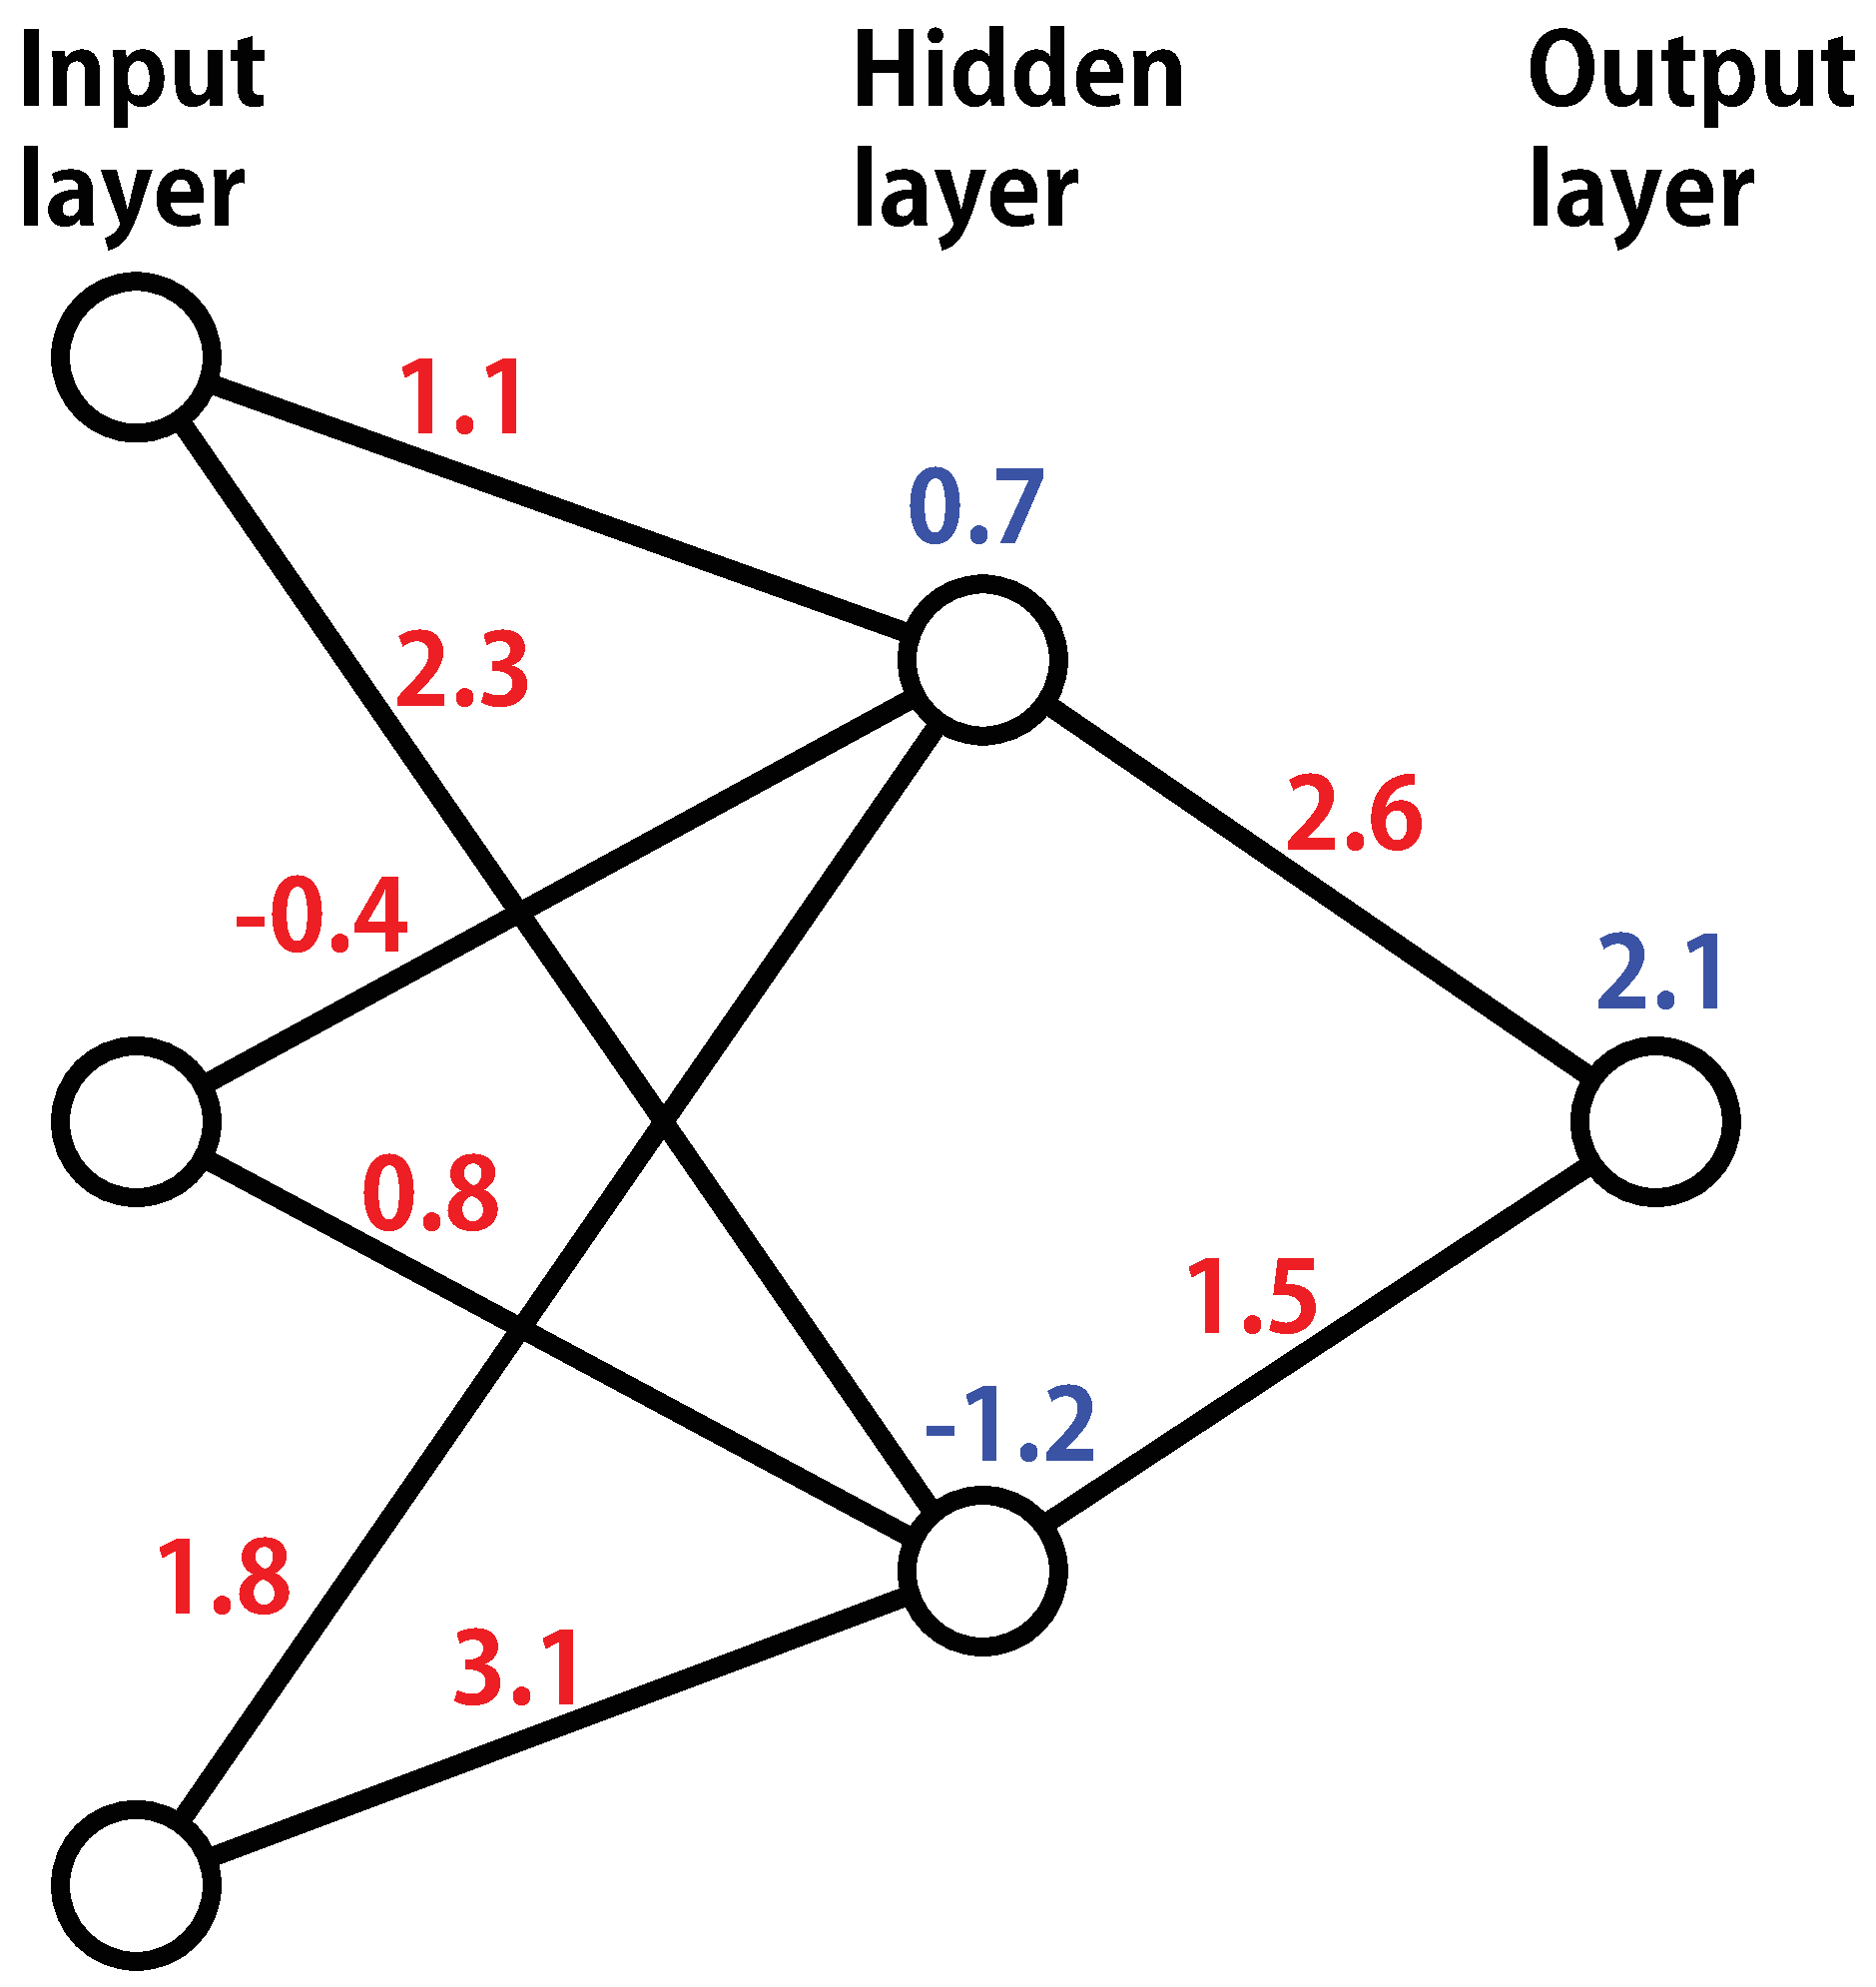
\includegraphics[width = 0.4 \textwidth]{./fig/ANN_sample_en}
  \caption{An example of an ANN.
    A red value indicates a weight, whereas
    a blue value indicates a bias.
    The direction of each arc is from left to right.}
  \label{fig:sample}
\end{figure}

\paragraph{Layers of an ANN.}
In the multi-layered perceptron model of ANNs,
an ANN consists of several \emph{layers}.
%
\begin{itemize}
  \item 
  The first layer is the {\em input layer}.
    Each node in the input layer is associated with a dimension of
    a feature vector (i.e., a descriptor). 
    Then the number of nodes in the input layer
    is equal to the number of dimensions of a feature vector. 
    
  \item 
  The subsequent layers (except the last one) are called
    {\em hidden layers}. A node in a hidden layer outputs a value
    based on the input values, where the input values
    are the outputs of all nodes in the previous layer.
    
  \item 
  The last layer is the {\em output layer} that has only one node.
    The output of this node is regarded as the output of the ANN. 
\end{itemize}

In the ANN of \figref{sample}, the input layer has three nodes.
This means that a feature vector should be have three dimensions as well.
The ANN has one hidden layer that has two nodes.
The output layer has exactly one node. 

\paragraph{Weights.}
In ANNs, each edge is assigned a numerical value, called a {\em weight}.
The weights are determined by \emph{training} the ANN, 
based on the given data set. 

In \figref{sample}, the weights of edges are indicated in red. 


\paragraph{Biases.}
In ANNs, each node in the hidden layers and the output layer
is assigned a numerical value, which is called a {\em bias}.
The biases are determined together 
with the weight by training the ANN based on the given data set. 

In \figref{sample}, the biases of nodes are indicated in blue. 



\paragraph{Activation function.}
In ANNs, each node except the output one is assigned an activation function.
This function computes the output of the node
according to the weighted sum of the input values minus the bias of the node.

In this project, we use the Rectified Linear-Unit (ReLU) function
for the activation function of each node in the hidden layers.
This choice is due to Module 3, 
where it is assumed that the ReLU function is used
as an activation function for ANNs in Module 2.

\medskip

The process of deciding (appropriate) weights and biases
from a given data is called a {\em learning}.


\subsection{Files in the package}
\tabref{files} shows the list of files in the package of Module 2. 

\begin{table}[h!]
  \centering
  \caption{List of files in the package of Module 2}
  \label{tab:files}
  \begin{tabular}{lcll}
  \hline
  \bf File &\ \ & \multicolumn{2}{l}{\bf Description}\\
  \hline
  \verb|mol-infer_ANN.py| && \multicolumn{2}{l}{A Python script to train an ANN}\\
  &&\multicolumn{2}{l}{\bf (To proceed to Module 3,}\\
  &&\multicolumn{2}{l}{\bf it is necessary to run this script)}\\
  &&\multicolumn{2}{l}{$\bullet$ Used non-standard libraries: {\tt numpy, pandas, scikit-learn}}\\
  \hline
  \verb|predict_values.py| && \multicolumn{2}{l}{A supplementary Python script}\\
  &&\multicolumn{2}{l}{that predicts the value of a chemical property}\\
  &&\multicolumn{2}{l}{for molecules in a given data set}\\
  &&\multicolumn{2}{l}{(It is not necessary to run this script)}\\
  &&\multicolumn{2}{l}{$\bullet$ Used non-standard libraries: {\tt numpy, pandas}}\\
  \hline
  %\multicolumn{4}{l}{\tt Manual\_Module\_2\_Cyclic\_jp.pdf}\\
  %\multicolumn{4}{l}{\tt Manual\_Module\_2\_Cyclic\_jp.tex}\\
  \multicolumn{4}{l}{\tt Manual\_Module\_2\_Cyclic\_improved\_jp.pdf}\\
  \multicolumn{4}{l}{\tt Manual\_Module\_2\_Cyclic\_improved\_jp.tex}\\
  \multicolumn{4}{l}{\tt fig/ANN\_sample\_jp.eps}\\
  &&\multicolumn{2}{l}{PDF, \LaTeX\  source of the manual}\\
  &&\multicolumn{2}{l}{and the image file (Japanese version)}\\
  \hline
  %\multicolumn{4}{l}{\tt Manual\_Module\_2\_Cyclic\_en.pdf}\\
  %\multicolumn{4}{l}{\tt Manual\_Module\_2\_Cyclic\_en.tex}\\
  \multicolumn{4}{l}{\tt Manual\_Module\_2\_Cyclic\_improved\_en.pdf}\\
  \multicolumn{4}{l}{\tt Manual\_Module\_2\_Cyclic\_improved\_en.tex}\\
  \multicolumn{4}{l}{\tt fig/ANN\_sample\_en.eps}\\
  &&\multicolumn{2}{l}{PDF, \LaTeX\   source of the manual}\\
  &&\multicolumn{2}{l}{and the image file (English version)}\\
  \hline
  \multicolumn{4}{l}{\bf Data files for BP (boiling point)~\cite{pubchem}}\\
  \multicolumn{2}{l}{\tt data/BP.sdf} & \multicolumn{2}{l}{SDF file containing molecule data.}\\
  \multicolumn{2}{l}{\tt } & \multicolumn{2}{l}{This file is not explicitly treated in Module 2.}\\
  \multicolumn{2}{l}{\tt data/BP\_fv.csv} & \multicolumn{2}{l}{File containing feature vectors}\\
  \multicolumn{2}{l}{\tt } & \multicolumn{2}{l}{that are obtained by applying Module 1 to {\tt BP.sdf}}\\
  \multicolumn{2}{l}{\tt data/BP\_value.csv} & \multicolumn{2}{l}{File containing BP values of molecules}\\
  \multicolumn{2}{l}{\tt data/BP\_ANN.LOG} & \multicolumn{2}{l}{Log of executing {\tt mol-infer\_ANN.py}}\\
  \multicolumn{2}{l}{\tt } & \multicolumn{2}{l}{for the data set that consists of {\tt BP\_fv.csv, BP\_value.csv}}\\
  \multicolumn{4}{l}{\tt data/BP\_ANN\_biases.txt} \\
  \multicolumn{4}{l}{\tt data/BP\_ANN\_weights.txt} \\
  &&\multicolumn{2}{l}{The biases and weights of the constructed NN}\\
  \hline
  \end{tabular}
\end{table}

\newpage

\begin{table}[t!]
  \centering
  (Cont. of \tabref{files})
  
  \begin{tabular}{lcll}
  \hline
  \bf File &\ \ & \multicolumn{2}{l}{\bf Description}\\
  \hline
  \multicolumn{4}{l}{\bf Data files for HC (heat of combustion)~\cite{pubchem}}\\
  \multicolumn{2}{l}{\tt data/HC.sdf} & \multicolumn{2}{l}{(All are analogous to BP)}\\
  \multicolumn{2}{l}{\tt data/HC\_fv.csv} \\%& \multicolumn{2}{l}{Module 1 に{\tt HC.sdf}を入力して生成した特徴ベクトル}\\
  \multicolumn{2}{l}{\tt data/HC\_value.csv} \\%& \multicolumn{2}{l}{化合物のHC値を記したファイル}\\
  \multicolumn{2}{l}{\tt data/HC\_ANN.LOG} \\%& \multicolumn{2}{l}{{\tt HC\_fv.csv, HC\_value.csv}から成る訓練集合に対して}\\
  %&&\multicolumn{2}{l}{{\tt mol-infer\_ANN.py}を実行し, 学習したときのログ出力}\\
  \multicolumn{4}{l}{\tt data/HC\_ANN\_biases.txt} \\
  \multicolumn{4}{l}{\tt data/HC\_ANN\_weights.txt} \\
  %&&\multicolumn{2}{l}{学習されたNNにおける各ノードのバイアス, }\\
  %&&\multicolumn{2}{l}{および各枝の重み}\\
  \hline
  \multicolumn{4}{l}{\bf Data files for KOW (log Kow)~\cite{pubchem}}\\
  \multicolumn{2}{l}{\tt data/KOW.sdf} & \multicolumn{2}{l}{(All are analogous to BP)}\\
  \multicolumn{2}{l}{\tt data/KOW\_fv.csv} \\%& \multicolumn{2}{l}{Module 1 に{\tt KOW.sdf}を入力して生成した特徴ベクトル}\\
  \multicolumn{2}{l}{\tt data/KOW\_value.csv} \\%& \multicolumn{2}{l}{化合物のKOW値を記したファイル}\\
  \multicolumn{2}{l}{\tt data/KOW\_ANN.LOG} \\%& \multicolumn{2}{l}{{\tt KOW\_fv.csv, KOW\_value.csv}から成る訓練集合に対して}\\
  %&&\multicolumn{2}{l}{{\tt mol-infer\_ANN.py}を実行し, 学習したときのログ出力}\\
  \multicolumn{4}{l}{\tt data/KOW\_ANN\_biases.txt} \\
  \multicolumn{4}{l}{\tt data/KOW\_ANN\_weights.txt} \\
  %&&\multicolumn{2}{l}{学習されたNNにおける各ノードのバイアス, }\\
  %&&\multicolumn{2}{l}{および各枝の重み}\\
  \hline
  \multicolumn{4}{l}{\bf Data files for MP (melting point)~\cite{pubchem}}\\
  \multicolumn{2}{l}{\tt data/MP.sdf} & \multicolumn{2}{l}{(All are analogous to BP)}\\
  \multicolumn{2}{l}{\tt data/MP\_fv.csv} \\%& \multicolumn{2}{l}{Module 1 に{\tt MP.sdf}を入力して生成した特徴ベクトル}\\
  \multicolumn{2}{l}{\tt data/MP\_value.csv} \\%& \multicolumn{2}{l}{化合物のMP値を記したファイル}\\
  \multicolumn{2}{l}{\tt data/MP\_ANN.LOG} \\%& \multicolumn{2}{l}{{\tt MP\_fv.csv, MP\_value.csv}から成る訓練集合に対して}\\
  %&&\multicolumn{2}{l}{{\tt mol-infer\_ANN.py}を実行し, 学習したときのログ出力}\\
  \multicolumn{4}{l}{\tt data/MP\_ANN\_biases.txt} \\
  \multicolumn{4}{l}{\tt data/MP\_ANN\_weights.txt} \\
  %&&\multicolumn{2}{l}{学習されたNNにおける各ノードのバイアス, }\\
  %&&\multicolumn{2}{l}{および各枝の重み}\\
  \hline
  \end{tabular}

\end{table}


%%%%%%%%%%%%%%%%%%%%%%%%%%%%%%%%%%%%%%%%%%%%%%%%%%%%%%%%%%%%
\clearpage
\section{A Quick Start}
\label{sec:quick}

\paragraph{Training an ANN.}
The following command constructs an ANN from the dataset such that
\begin{itemize}
\item the set of feature vectors is written in \verb|data/BP_fv.csv|; and
\item the set of property values (BP in this case) is written in \verb|data/BP_value.csv|
\end{itemize}
\begin{oframed}
{\small
\verb|$ python mol-infer_ANN.py data/BP_fv.csv data/BP_value.csv output 20 10|
% \hfill $(\clubsuit)$
}
\end{oframed}

The constructed NN has two hidden layers,
where the numbers of nodes in these layers
are 20 and 10, respectively.
The weights of arcs are output to the file \verb|output_weights.txt|
and the biases of nodes are output to the file
\verb|output_biases.txt|.  
%
{\bf The files containing weights and biases are used in Module~3}. 


\paragraph{Predicting the property value of a given molecule.}
The property value of a molecule can be predicted by using a trained ANN.

The following command invokes a Python  script that
reads the information (edge weights and node biases)
of a trained ANN, and then uses each of the feature vectors
given in the file \verb|data/BP_fv.csv| as input to the
ANN's prediction function.
The edge weights of the trained ANN are read from the file \verb|output_weights.txt|,
and node biases are read from the file \verb|output_biases.txt|.
The output results 
are written to the file \verb|predicted.txt|. 

\begin{oframed}
  {\small
\noindent The symbol $\backslash$ at the end of the first line indicates that there
is no line break between the two lines, that is, they should be input without 
pressing the ``enter'' key.
\begin{verbatim}
$ python predict_values.py output_weights.txt output_biases.txt \
    data/BP_fv.csv predicted.txt
\end{verbatim}
}
  \end{oframed}

\begin{itemize}
\item Given an SDF file,
  one can generate the feature vectors of the molecules in the SDF
  by using the program in Module 1.
%\item 上のコマンドは, さらに上のコマンド$(\clubsuit)$で\verb|data/BP_fv.csv|を
%  特徴ベクトルとした訓練集合から学習したニューラルネットワークに関する \verb|output_weights.txt|および \verb|output_biases.txt|を用いるものとみなせば, 
%  訓練集合自身の化学的性質の値を推定していることになる. 
\item This script is supplementary, and it is not directly used in Modules~3 and~4. 
\end{itemize}


\section{Details in the Input and Output of the Program}
\label{sec:io}

\subsection{Input}
\subsubsection{Feature vectors}
The feature vectors should be written in
a so-called {\bf FV format} to
a csv (comma-separated value) file. 
%
The feature vector generator in Module~1
generates a csv file in the FV format
from a given SDF.
As long as one uses the csv file generated in Module 1,
no problem should occur in Module 2. 

We explain the structure of the FV format using a simple example.  
\begin{oframed}
  {\small
\begin{verbatim}
CID,n,cs,ch,nsH
244,8,6,2,8
307,10,6,4,8
657014,11,7,1,18
16704,9,9,0,10
\end{verbatim}
}
\end{oframed}
\begin{itemize}
\item In the first line, the descriptor names should be written in comma-separated style.  
\item The first descriptor {\bf must be} CID (Compound ID).
  The CID values are not used to train an ANN, just for identification. 
\item In the above example,
  four descriptors are introduced: 
  \verb|n| (the number of atoms except hydrogens),
  \verb|cs| (core-size),
  \verb|ch| (core-height), and
  \verb|nsH| (the number of hydrogens). 
\item In each of the subsequent lines,
  the CID and the feature vector of one molecule
  should be specified in comma-separated style. 
\item The molecules {\bf need not be} ordered according to CID. 
\end{itemize}


\subsubsection{Property values}
The property values should be described in a csv file as follows.  
\begin{oframed}
  {\small
\begin{verbatim}
CID,a
307,11.2
244,-0.5
657014,98.124
16704,-12.8
117,5.3
\end{verbatim}
}
\end{oframed}
\begin{itemize}
\item {\bf The first line should be \verb|CID,a|. }
\item In each of the subsequent lines,
  CID and the property value of one molecule
  should be written in comma-separated style. 
\item The molecules need not be ordered with respect to CID. 
\end{itemize}
  
  
\subsection{Execution}

We use the Python script {\tt mol-infer\_ANN.py}
to train an ANN, as outlined in \secref{quick}.


\subsubsection{Arguments}
We here revisit the commands 
explained in \secref{quick}.
\begin{oframed}
{\small
\verb|$ python mol-infer_ANN.py data/BP_fv.csv data/BP_value.csv output 20 10|
}
\end{oframed}
The meaning of each of the command-line parameters is as follows:
\begin{itemize}
\item Parameter~1: 
  A csv file the stores the feature vectors of chemical compounds,
  
\item Parameter~2: 
  A csv file that stores observed values of a chemical property/activity of chemical compounds,
  
\item Parameter~3: 
Filename where the weights and biases of a trained ANN will be stored,

\item Parameter~4: 
The number of nodes of hidden layers in the ANN, each layer separated by a space.
\end{itemize}

If the Python script is invoked without supplying command-line arguments,
or in the case that there is a significant error in the arguments,
then a brief description of the command-line parameters will be printed.
\begin{oframed}
A verbatim output of the output of the program when invoked without any command-line parameters. The backslash symbol (\verb|\|) indicates that there is no actual line break. 
  {\small
\begin{verbatim}
$ python mol-infer_ANN.py 

usage: mol-infer_ANN.py (TrSet_FeatureVector.csv)(TrSet_TargetValue.csv) \
	    (Output_Name)(NN_Architecture)
                  
  - TrSet_FeatureVector.csv ... \
      The CSV file generated by our feature vector generator in Module 1.
  - TrSet_TargetValue.csv ... \
      The CSV file that contains target values.
    = The first column must contain CIDs.
    = The second column must contain target values and be named 'a'. 
    = All CIDs appearing in TrSet_FeatureVector.csv must be contained in \
	      TrSet_TargetValue.csv. 
  - OutputName_{biases,weights}.txt will be output. \
      They contain data on the constructed ANN. 
  - NN_Architecture ... Number of nodes in hidden layer(s).
\end{verbatim}
  }
  \end{oframed}

If the program is invoked with a proper set of command-line parameters,
then the training process of an ANN will begin.

To evaluate the performance of the trained ANN,
we use 5-fold cross-validation.
The ANN that achieved the highest coefficient of determination 
(${\rm R}^2$ score) for the test set over the five trials
is selected, and its weights and biases are stored
in a file.
Using the above example of parameter values,
where the value of parameter 3 is set to be \verb|output|,
the following two files will be written to disk:
\begin{itemize}
\item \verb|output_weights.txt| (stores the weights)
\item \verb|output_biases.txt| (stores the biases)
\end{itemize}
These two files are necessary in Module 3.


\paragraph{Caution on the data set}
The training set for training the ANN is given 
in the following two files
%
\begin{itemize}
\item a csv file with feature vectors of chemical compounds, and 
\item a csv file with observed values for a chemical property/activity.
\end{itemize}
Both files include the CID number of the corresponding chemical compound.
One important point to note is that
%
\begin{center}
  {\bf each of the CIDs in the former file must appear in the latter }
\end{center}
%
however, the opposite is not enforced.
In other words, there might be a chemical compound
for which an observed value of some property/activity
is listed in the latter file, but whose
feature vector is not included in the former.
Such values will be silently ignored.


\subsubsection{Hyper-parameters}

We use the Python  library {\tt scikit-learn}\footnote{\url{https://scikit-learn.org/stable/}}
and its {\tt MLPRegressor} tool
to do the training of an ANN as
a multi-layered perceptron.
After line 133 in the Python script 
\verb|mol-infer_ANN.py|, an instance of 
an \verb|MLPRegressor| is initialized, 
and its hyperparameters can be changed at this point.
Some of the various parameters are set as follows:
\begin{itemize}
\item \verb|activation|: \verb|`relu'|  \\
{\color{red}{\bf Attention:} 
If the trained neural network is to be used in Module 3 and afterward, 
the only possible choice here is
\verb|`relu'| (Rectified Linear Unit Function - ReLU).}
\item \verb|alpha|: $10^{-5}$
\item \verb|early_stopping|: \verb|False|
\item \verb|hidden_layer_sizes|: Passed as a command-line parameter at invocation
\item \verb|max_iter|: $10^{10}$
\item \verb|random_state|: 1
\item \verb|solver|: \verb|`adam'|
\end{itemize}


\subsection{Output}

We revisit the command issued as below, 
and explain the resulting output.
\begin{oframed}
{\small
\verb|$ python mol-infer_ANN.py data/BP_fv.csv data/BP_value.csv output 20 10|
}
\end{oframed}

\subsubsection{Standard output}

When the above command is issued on the command prompt,
the results of the computation process will be displayed on the 
standard output.
An example of this output is stored in the file
\verb|data/BP_ANN.LOG| which is included together with
the program package and this note.
\begin{oframed}
  {\small
\begin{verbatim}
src/preparation/BP_fv.csv contains 181 vectors for 107 (=CID+106) features.
src/preparation/BP_value.csv contains 230 target values.
n range = [5,30]
a range = [31.5,470.0]
#instances = 181
#features = 106

D1: train 144, test 37
training time: 3.187196731567383
R2 score train = 0.9935319077425955
R2 score test = 0.7855694851759929
R2 score all = 0.9599908495442584
MAE score train = 3.8570127089010384
MAE score test = 19.756408746147212
MAE score all = 7.10716548999556

D2: train 145, test 36
training time: 5.0139079093933105
R2 score train = 0.9930416804444452
R2 score test = 0.6390572625074291
R2 score all = 0.9339056805642507
MAE score train = 3.7281172621746888
MAE score test = 27.996544836634186
MAE score all = 8.554986834995363

D3: train 145, test 36
training time: 4.264358758926392
R2 score train = 0.9961346879653636
R2 score test = 0.8566979846124056
R2 score all = 0.9637772344809027
MAE score train = 2.870368503215682
MAE score test = 22.925217956024927
MAE score all = 6.8591783391335435

D4: train 145, test 36
training time: 2.9935202598571777
R2 score train = 0.9909067339023991
R2 score test = 0.8390994594153819
R2 score all = 0.9669036994338265
MAE score train = 4.470398694611737
MAE score test = 18.691072072382227
MAE score all = 7.298819918919681

D5: train 145, test 36
training time: 4.9648661613464355
R2 score train = 0.9946933391220482
R2 score test = 0.8479544758088942
R2 score all = 0.9574271159388575
MAE score train = 3.352287445970431
MAE score test = 21.80973582058148
MAE score all = 7.023382150312958
0.9935319077425955 0.7855694851759929 0.9599908495442584 3.187196731567383
0.9930416804444452 0.6390572625074291 0.9339056805642507 5.0139079093933105
0.9961346879653636 0.8566979846124056 0.9637772344809027 4.264358758926392
0.9909067339023991 0.8390994594153819 0.9669036994338265 2.9935202598571777
0.9946933391220482 0.8479544758088942 0.9574271159388575 4.9648661613464355
Average time = 4.08476996421814
Average R2 test score = 0.7936757335040208
Average MAE test score = 22.235795886354005
  \end{verbatim}        
}
\end{oframed}

\begin{itemize}
\item  
First, the number of feature vectors, as well as the
number of descriptors are output.
Next comes the range 
(\verb|n range|, in the above example 5 -- 30)
of the number of non-hydrogen atoms (descriptor \verb|n|)
in the chemical
compounds in the training set, 
followed by the range 
(\verb|a range|,  31.5 -- 470.0 above)
of the observed 
chemical property/activity in the training data
(in this case, boiling point).

\item 
Following, the summary of each of the five runs of the
5-fold cross-validation is printed.

\item
Finally, the average of the calculation time,
R$^2$ score of the test set and MAE score of the test set over the 
five folds are printed.

\item 
In the above example, the ANN constructed 
in the third of the five folds had the 
highest R$^2$ score of 0.856697$\dots$, 
and therefore the values of its weights and
biases are written in the files
\verb|output_weights.txt| and \verb|output_biases.txt|, respectively.

\item
Note that a copy of each of the above files, 
\verb|output_weights.txt| and \verb|output_biases.txt|, 
is included in the set of files together with this note.
\end{itemize}


\subsubsection{Edge weights}
Following we explain the contents of the file
\verb|mol-infer_ANN.py|
that contains the values of the weights of the ANN.


For simplicity, let us assume that the ANN depicted
in \figref{sample} has been obtained after training.
The contents of the file with the weights of this ANN
would be as follows.
%
\begin{oframed}
{\small
\begin{verbatim}
3 2 1
1.1 2.3
-0.4 0.8
1.8 3.1
2.6
1.5
\end{verbatim}
}
\end{oframed}
%
\begin{itemize}
\item 
The first row gives the architecture of the ANN,
that is the number of nodes in each of its layers.
starting with the input layer, then the hidden layers, and
finally the output layer.

\item 
Starting from the second line and onward,
follow the weights of the ANN.
Each row gives the weights of the edges going out of a single node.
\end{itemize}


\subsubsection{Biases of nodes}
In a similar manner,
we give an explanation of the file that contains the
biases of the ANN obtained
by executing the Python script \verb|mol-infer_ANN.py|.

For sake of simplicity, again consider
the ANN depicted in \figref{sample}.
The values for the node biases of this ANN would be given as follows.
%
\begin{oframed}
{\small
\begin{verbatim}
0.7
-1.2
2.1
\end{verbatim}
}
\end{oframed}
Each row contains the bias value of a single node.
Note that the nodes of the output layer do not have biases.

\begin{thebibliography}{9}
\bibitem{pubchem} HSDB in 
PubChem \url{https://pubchem.ncbi.nlm.nih.gov} (accessed on February 1st, 2021)
\end{thebibliography}


\end{document}
%%%%%%%%%%%%%%%%%%%%%%%%%%%%%%%%%%%%%%%%%%%%%%%%%%%%%%%%%%%%
%%%%%%%%%%%%%%%%%%%%%%%%%%%%%%%%%%%%%%%%%%%%%%%%%%%%%%%%%%%%
%%%%%%%%%%%%%%%%%%%%%%%%%%%%%%%%%%%%%%%%%%%%%%%%%%%%%%%%%%%%

